% ============================================================================
% OUP Bioinformatics (bioinfo.cls) formatted submission
% formatting/template compliance + figure alt text added.
% ============================================================================

\documentclass{bioinfo}

\usepackage{amsmath,amsfonts,amssymb}
\usepackage{graphicx}
\usepackage{hyperref}
\usepackage{booktabs}
\usepackage{tikz}
\usepackage{pdfcomment}
\usepackage{orcidlink}
\usepackage{float}

% Standardized math commands
\newcommand{\R}{\mathbb{R}}
% Redefine \Description to create a transparent tooltip over the image
\renewcommand{\Description}[1]{\pdftooltip{\rule{0pt}{0pt}}{#1}}

\usetikzlibrary{shapes.geometric, arrows.meta, positioning, calc, backgrounds, fit}

% Alt-text support (safe fallback if \Description is not provided by the template/toolchain)
\providecommand{\Description}[1]{}

\begin{document}

\firstpage{1}

\title[FuseLens]{FuseLens: Attention-Guided Chimeric Transcripts Classification via Long-Context Genomic AI Foundation Models}
\author{
Udi Bahat\textsuperscript{1},
Alon Kipnis\textsuperscript{1},
Sarel Cohen\textsuperscript{1},
Dylan D'Souza\textsuperscript{4},
Milana Frenkel-Morgenstern\textsuperscript{2,3}}
\address{\textsuperscript{1}Efi Arazi School of Computer Science, \textsuperscript{2}Scojen Institute of Synthetic Biology, \textsuperscript{3}Dina Recanati School of Medicine; Reichman University. \textsuperscript{4}The Azrieli Faculty of Medicine, Bar Ilan University.\\  
ubahat@post.runi.ac.il, \{alon.kipnis, sarel.cohen, milana.morgenstern\}@runi.ac.il, dylan.dsouza@biu.ac.il}
\maketitle
\begin{abstract}
\textbf{Motivation:} Chimeric transcripts are hybrid RNA molecules generated by chromosomal rearrangements or transcriptional read-through events. Their detection has become a central task in cancer genomics, as chimeric RNAs represent expressed, functional biomarkers and actionable therapeutic targets. However, candidate fusion transcripts identified by high-throughput discovery pipelines are often noisy, necessitating accurate post hoc validation. We introduce \textit{FuseLens}, a sequence-based classifier for chimeric transcripts designed to address this challenge through three core capabilities: scalable long-context modeling, homology-aware adversarial training, and attention-derived weak localization. FuseLens processes 32\,kb sequence windows at single-nucleotide resolution using sub-quadratic long-convolution operators and employs a learnable attention pooling head to jointly perform classification and breakpoint proxy localization.

\textbf{Results:} Evaluated on a curated dataset of 187{,}925 genomic windows, FuseLens achieves strong discriminative performance (accuracy 0.9162, AUC =0.9736). Post hoc analysis of true positive predictions reveals variable-resolution localization behavior: while the mean attention width is 6{,}138\,bp, the median width is substantially narrower at 1{,}911\,bp, indicating that the model frequently concentrates attention near the structural breakpoint ($\sim$6\% of the input window).

\textbf{Availability and Implementation:} The implementation is available at \href{https://github.com/UdiRuni/FuseLens}{https://github.com/UdiRuni/FuseLens}, including data construction pipelines, augmentation operators, model architecture, and evaluation scripts.

\textbf{Contact:} Milana
Frenkel-Morgenstern; Udi Bahat \\
milana.morgenstern@runi.ac.il; ubahat@post.runi.ac.il
\end{abstract}

\section{Introduction}
Gene fusions are hybrid genes formed by chromosomal re\-arrange\-ments at the DNA level, while chimeric transcripts are their expressed RNA products~\cite{chimeras_shape}. Chimeric RNAs constitute direct, functional biomarkers in cancer cells and play a central role in oncogenesis and therapeutic targeting. Approximately 20\% of human cancers are associated with gene fusion events~\cite{mitelman2007impact}. Canonical examples include \textit{BCR-ABL1} in chronic myeloid leukemia~\cite{bcr_abl}, which is effectively targeted by tyrosine kinase inhibitors~\cite{imatinib}. Accurate identification of RNA chimeras is therefore critical for both diagnosis and treatment selection. However, discovery pipelines often generate large numbers of candidates, many of which represent artifacts or benign transcriptional events. Reliable, high-precision sequence-level classifiers are thus required to automate fusion validation and reduce the burden of manual curation~\cite{chitars_db}.
\subsection{The Biological Constraint}
A fundamental challenge in modeling gene fusions is the scale mismatch between biological features and computational context windows. The median human gene length is approximately 26\,kb \cite{gene_length_stats}, and pathogenic breakpoints often reside deep within vast intronic regions. Furthermore, for transcription-induced chimeras (cis-SAGe), the median intergenic distance between fusion partners is $\sim$8.5\,kb \cite{giacomini2013}, meaning a single fusion event might span a genomic territory exceeding 60\,kb. 

\subsection{Previous Works}
Tools such as STAR-Fusion \cite{starfusion} and Arriba \cite{arriba} rely on short-read alignment signatures (e.g., split reads and discordant pairs). While effective, alignment-first pipelines may produce false positives in low-complexity regions, paralogous loci, or in the presence of sequencing artifacts \cite{fusion_challenges}, and might not explicitly learn long-range sequence context around candidate junctions.

\subsection{Sequence-First Architectures}
Deep learning provides a complementary ``sequence-first'' approach to analyze raw nucleotide sequence directly to capture discriminative genomic grammar—a necessity increasingly emphasized by broader clinical benchmarks \cite{krupicka2025benchmarking}. Early CNN-based approaches (e.g., FusionAI \cite{fusionai}) demonstrated the feasibility of this paradigm but were constrained by limited receptive fields. Transformer-based approaches, such as DNABERT \cite{dnabert} and Nucleotide Transformer \cite{nucleotide}, capture global context but incur quadratic attention costs ($O(n^2)$) \cite{vaswani}, making the modeling of single-position interactions over tens of kilobases computationally expensive.

\subsection{FuseLens}
FuseLens processes 32\,kb windows and is inherently scalable up to 1 million base pairs via sub-quadratic ($O(n\log n)$) implicit long convolutions \cite{hyena_hierarchy}. To capture sparse breakpoint signals without the dilution inherent in standard global pooling, we employ a linear-time attention pooling head that outputs a distribution over positions.
We use the peak (or a high-mass interval) as a \emph{localization proxy} under confidence gating.
We emphasize that these attention weights are learned pooling coefficients and are not guaranteed to be an explanation of the prediction; therefore, we report them as an approximate, weakly supervised pointer signal rather than definitive coordinates. \cite{attention_not_explanation, attention_not_not}.

\subsection{Contributions}
FuseLens integrates three components to enable high-precision detection of chimeric transcripts:
\begin{itemize}
   \item \textbf{Long-context sequence classification:} We present, to our knowledge, the first application of implicit long-convolution foundation models (HyenaDNA~\cite{hyenadna}) to chimeric transcript detection. The model processes 32\,kb genomic windows at single-nucleotide resolution with sub-quadratic complexity, enabling the capture of long-range dependencies relevant to fusion grammar.

   \item \textbf{Adversarial negative curation:} We introduce a principled negative data construction strategy designed to decouple gene identity from structural fusion signals. By training against engineered hard negatives---including shift-invariant junctions ($\mathcal{J}$) and reverse-complement decoys ($\mathcal{RC}$)---the model is forced to learn structural fusion grammar rather than memorizing specific gene sequences.

   \item \textbf{Weakly supervised localization and interpretability:} We demonstrate a linear-complexity attention pooling mechanism that functions both as a discriminative classifier and as a soft localization operator, yielding approximate breakpoint regions (median resolution $\sim$2\,kb) using only sequence-level binary supervision. In addition to supporting automated filtering, this attention-derived signal provides an \emph{interactive} exploratory cue, enabling practitioners to inspect, prioritize, and contextualize candidate fusion regions during downstream analysis.

\end{itemize}
\section{Biological Background}
\subsection{Mechanisms of Formation}
Chimeric transcripts arise through distinct mechanisms \cite{chimeras_shape}. The most prominent class involves \textit{chromosomal rearrangements}, characterized by the physical breaking and rejoining of DNA via inversions (e.g., \textit{EML4-ALK}) or inter-chromosomal translocations (e.g., \textit{BCR-ABL1}). Beyond genomic rearrangements, chimeras may also form through \textit{Read-Through (Cis-SAGe)}, where transcriptional machinery ignores termination signals between adjacent genes in the absence of DNA modification \cite{slc45a3_elk4}. A third category includes \textit{Cis-Type SV-driven fusions}, which result from local structural variations—such as deletions or duplications—that bring distinct loci into contiguity. Distinguishing these physiological events is a critical challenge for high-precision clinical classifiers.
\subsection{Examples of Key Oncogenic Fusions}
A primary example is \textit{BCR-ABL1} in Chronic Myeloid Leukemia (CML), resulting from the t(9;22) translocation (Philadelphia Chromosome), which creates a constitutively active tyrosine kinase \cite{bcr_abl}. In solid tumors, \textit{TMPRSS2-ERG} is found in approximately 50\% of prostate cancers, where the androgen-responsive promoter of \textit{TMPRSS2} fuses with the oncogene \textit{ERG} \cite{tmprss2_erg}. Additionally, non-genomic mechanisms such as \textit{SLC45A3-ELK4}, a prominent example of \textit{cis-splicing} in prostate cancer that can form via transcriptional read-through without any underlying DNA mutation \cite{slc45a3_elk4}.

\section{Methodology}

\subsection{Problem Formulation and Scope}
FuseLens addresses \textbf{fusion-candidate window classification}. The input is a variable-length sequence window candidate (e.g., fusion caller output, database curation, or structural variant hypotheses).

\subsection{FuseLens Model Architecture}
\begin{figure}[H]
\centering
\Description{Block diagram of FuseLens: sequence window input, HyenaDNA embeddings, attention pooling and weighted sum, classifier producing fusion probability and breakpoint proxy.}
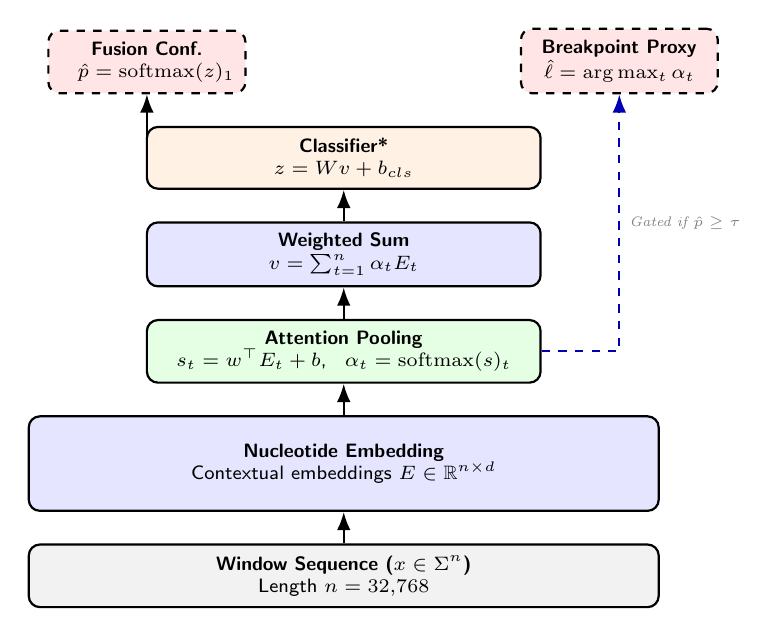
\begin{tikzpicture}[
    font=\sffamily\scriptsize,
    node distance=0.4cm and 1.0cm,
    % Optional: Reduced box size slightly to match smaller text
    box/.style={draw, rounded corners, minimum width=3.5cm, minimum height=0.7cm, align=center, line width=0.8pt, inner sep=4pt},
    process/.style={box, fill=blue!10},
    decision/.style={box, fill=green!10},
    output/.style={box, fill=red!10, dashed},
    arrow/.style={-Latex, thick},
    labeltext/.style={font=\tiny\itshape, text=gray}
]
    \node (input) [box, fill=gray!10, minimum width=8cm] {\textbf{Window Sequence ($x\in\Sigma^n$)}\\ Length $n=32{,}768$};

    \node (hyena) [process, above=of input, minimum height=1.2cm, minimum width=8cm] {\textbf{Nucleotide Embedding}\\ Contextual embeddings $E \in \mathbb{R}^{n \times d}$};

    \node (attn) [decision, above=of hyena, minimum width=5cm] {\textbf{Attention Pooling}\\ $s_t=w^\top E_t+b$,\;\; $\alpha_t=\mathrm{softmax}(s)_t$};

    \node (pool) [process, above=of attn, minimum width=5cm] {\textbf{Weighted Sum}\\ $v=\sum_{t=1}^n \alpha_t E_t$};

    \node (clf) [box, fill=orange!10, above=of pool, minimum width=5cm] {\textbf{Classifier*}\\ $z=Wv+b_{cls}$}; 

    \node (prob) [output, above=of clf, xshift=-2.5cm, minimum width=2.5cm] {\textbf{Fusion Conf.}\\ \;\; $\hat{p}=\mathrm{softmax}(z)_1$};

    \node (loc) [output, above=of clf, xshift=3.5cm, minimum width=2.5cm] {\textbf{Breakpoint Proxy}\\ $\hat{\ell}=\arg\max_t \alpha_t$};

    \draw[arrow] (input) -- (hyena);
    \draw[arrow] (hyena) -- (attn);
    \draw[arrow] (attn) -- (pool);
    \draw[arrow] (pool) -- (clf);
    \draw[arrow] (clf.west) -| (prob.south);

    \draw[arrow, dashed, color=blue!70!black]
        (attn.east) -- (attn.east -| loc.south) -- node[midway, right, labeltext] {Gated if $\hat{p}\ge\tau$} (loc.south);
\end{tikzpicture}
\caption{\textbf{FuseLens architecture.} HyenaDNA produces contextual token embeddings, attention pooling aggregates evidence for classification, and the attention peak provides a localization proxy under confidence gating. *Classifier Training: minimize BCE  (see section 3.9).}
\label{fig:architecture}
\end{figure}
\subsection{Inputs}
Each sample $s$ is a variable-length sequence window
\begin{equation}
s \in \Sigma^{l}, \quad l \le 32{,}768
\end{equation}
where $\Sigma$ is the character alphabet $\{A,C,G,T\}$ used by the tokenizer.

\subsection{Data Processing Step}
To reduce positional shortcuts (e.g., ``junction always near the center''), we apply padding with \textbf{random jitter} to map $s$ into a fixed-length window $x\in\Sigma^n$, where $n = 32,768$:
\begin{equation}
\mathrm{Jitter}(s) =
\begin{cases}
r_L \oplus s \oplus r_R & \text{if } m < n\\
s_{k:k+n} & \text{if } m \ge n
\end{cases}
\end{equation}
where $m=|s|$ is the length of the core sequence, $|r_L|+|r_R|=n-m$, and $|r_L|\sim \mathrm{Unif}\{0,\dots,n-m\}$ (uniform random placement). If the sequence exceeds the window size ($m \ge n$), a random crop is taken at start index $k\sim \mathrm{Unif}\{0,\dots,m-n\}$. Padding strings $r_L, r_R$ are sampled IID from $\{A,C,G,T\}$.

\subsection{Nucleotide Embedding}
Given an input nucleotide sequence $u \in \mathbb{R}^{n \times c}$ (where $c = 4$), FuseLens utilizes the pretrained HyenaDNA model \cite{hyenadna} as a backbone feature extractor. We denote the function $\Phi$ that maps $u$ to a contextual embedding sequence $E$:
\begin{equation}
E = \Phi(u)
\end{equation}
where $E \in \mathbb{R}^{n \times d}$ and $d=256$ is the embedding dimension.

\subsection{Attention, Pooling vs. Standard Transformers}
Our architecture incorporates a pooling mechanism that adapts the mathematical principles of Transformers for efficient sequence aggregation. Unlike standard self-attention, which aims to contextualize features via pairwise token interactions ($O(N^2)$), our approach focuses on dimensionality reduction ($O(N)$).

We denote the specific embedding vector at the $t$-th nucleotide position as $E_t \in \mathbb{R}^d$. FuseLens computes a scalar importance score for each nucleotide embedding $E_t$, allowing it to differentiate between informative regions (e.g., breakpoints) and background noise. These scores are used to calculate a weighted sum of the feature sequence, compressing the temporal dimension into a single context vector. 
First, we compute an unnormalized scalar score (logit) $s_t$ for each nucleotide position $t$ via a learnable \textbf{linear projection}:
\begin{equation}
s_t = w^\top E_t + b
\end{equation}
where $w \in \mathbb{R}^d$ is a learnable weight vector that "scores" the embeddings, and $b \in \mathbb{R}$ is the scalar bias.
To derive the final attention weights $\alpha_t$, we apply the softmax function over the sequence length $n$:
\begin{equation}
\alpha_t = \frac{e^{s_t}}{\sum_{j=1}^{n}e^{s_j}}
\end{equation}
The final pooled sequence representation $v \in \mathbb{R}^{d}$ is the weighted sum:
\begin{equation}
v = \sum_{t=1}^{n}\alpha_t E_t
\end{equation}
The classifier then produces logits $z\in\mathbb{R}^2$, corresponding to the binary class scores (fusion vs. non-fusion):
\begin{equation}
z = Wv + b_{cls}
\end{equation}
where $W \in \mathbb{R}^{2 \times d}$ is a learnable weight matrix and $b_{cls} \in \mathbb{R}^2$ is the bias vector.
Finally, we calculate the fusion probability:
\begin{equation}
\hat{p} = \mathrm{softmax}(z)_1
\end{equation}
Here, $\hat{p} \in [0,1]$ denotes the confidence score for the positive (fusion) class.

\subsection{Confidence-gated weak localization}
\label{sec:localization}
We define the attention-peak location based on the maximum attention weight:
\begin{equation}
\hat{\ell} = \mathrm{argmax}_{t\in\{1,\dots,n\}}\alpha_t
\end{equation}
We only report localization if the model confidence exceeds a threshold $\tau$:
\begin{equation}
\hat{\ell}_{\text{final}} =
\begin{cases}
\hat{\ell} & \text{if } \hat{p}\ge\tau\\
\varnothing & \text{otherwise}
\end{cases}
\end{equation}

\subsection{Outputs}
FuseLens returns a fusion confidence score $\hat{p}$ estimating $P(y=1 \mid s)$ and a localization proxy $\hat{\ell}$ (described in Section \ref{sec:localization}). The final binary prediction $\hat{y}$ is determined by a decision threshold $\tau \in (0,1)$:
\begin{equation}
\hat{y} =
\begin{cases}
1 \, (\text{Positive}) & \text{if } \hat{p} \ge \tau \\
0 \, (\text{Negative}) & \text{if } \hat{p} < \tau
\end{cases}
\end{equation}
where $\tau$ is calibrated to attain a specific target false positive rate.
\subsection{Training Objective}
We optimize the model parameters $\theta = \{w, b, W, b_{cls}, \Phi_{weights}\}$ by minimizing the Binary Cross-Entropy (BCE) loss over our dataset :
\begin{equation}
\mathcal{L}(\theta) = -\frac{1}{N} \sum_{i=1}^{N} \left[ y_i \log(\hat{p}_i) + (1 - y_i) \log(1 - \hat{p}_i) \right]
\end{equation}
where $y_i \in \{0,1\}$ is the ground truth label and $\hat{p}_i$ is the predicted fusion probability for sample $i$. The inclusion of hard negatives (Section \ref{NegativeDataCuration}) ensures that the term $(1-y_i)$ heavily penalizes the model for assigning high confidence to non-chimeric decoys.
\subsection{Negative Data Curation}\label{NegativeDataCuration}
We define hard negatives as negative samples (non-fusions) that induce high loss values during training. Their inclusion prevents the model from relying on gene-identity heuristics and enforces learning of the specific fusion breakpoint signature.

Given a dataset of canonical sequences $S=\{s_1, \dots, s_N\}$ where $s_i \in \{A,C,G,T\}^L$ derived from UniProt Swiss-Prot \cite{uniprot_db}. We used reviewed Swiss-Prot entries as a high-confidence gene list and retrieved the corresponding canonical transcript/CDS nucleotide sequences from standard repositories via accession mapping, then applied three mathematical operators to generate ``Hard Negatives''.

\begin{enumerate}
    \item \textbf{Reverse Complement Operator ($\mathcal{RC}$):}\\
    Let $\mathcal{C}$ be the base-pairing function ($A \leftrightarrow T, C \leftrightarrow G$).
    \begin{equation}
        \mathcal{RC}(s_i) = (\mathcal{C}(b_L), \mathcal{C}(b_{L-1}), \dots, \mathcal{C}(b_1))
    \end{equation}
    This generates the sequence of the opposing DNA strand.  Since functional genomic motifs (e.g., splice sites, promoter regions) are strand-specific, this operator forces the model to learn the strict $5' \to 3'$ syntax of the coding transcript, distinguishing valid gene content from its non-coding complement.

    \item \textbf{Grammar Inversion Operator ($\mathcal{R}_{seq}$):}\\
    To generate decoys that preserve nucleotide composition but destroy biological syntax, we apply a strict sequence reversal \textit{without} complementation:
    \begin{equation}
        \mathcal{R}_{seq}(s_i) = (b_L, b_{L-1}, \dots, b_1)
    \end{equation}
    Unlike random shuffling, strict reversal preserves the overall base composition while disrupting orientation-dependent syntax (e.g., donor/acceptor ordering), encouraging the classifier to rely on higher-level grammar rather than simple composition.

    \item \textbf{Shift-Invariant Junction Operator ($\mathcal{J}$):}\\
    We implement a \textit{Circular Permutation} strategy on a single gene $s_i$:
    \begin{equation}
        \mathcal{J}(s_i, k) = s_i[k:L] \oplus s_i[1:k]
    \end{equation}
    where $k \sim \text{Unif}(0, L)$ and $\oplus$ denotes concatenation. This operator creates a ``decoy breakpoint'' (a discontinuity) and forces the model to search the entire 32\,kb window for anomalies. By introducing a structural break within a single gene, this penalizes the model for simply detecting "edges" or discontinuities, forcing it to verify that the fused segments are semantically incompatible (i.e., from different genes) rather than just interrupted.
\end{enumerate}

\subsection{Design Rationale and Validity of Synthetic Hard Negatives} To prevent shortcut learning, our negative operators are designed to decouple true fusion signals from low-level sequence statistics. First, we employ composition-matched sequence perturbations, a widely established baseline for genomic sequence models \cite{ushuffle, zeng_dinuc}, ensuring the model relies on structural motifs rather than k-mer frequency shifts. Second, we leverage the directionality of biological signals (e.g., splice grammar) by generating strand-inconsistent sequences via reverse-complement
 and random jitter \cite{evoaug}. Finally, our intra-gene circular permutation operator introduces non-colinear "junctions" within a single gene. This specifically mimics the back-splice junctions observed in circular RNAs (circRNAs)—a known confounder in clinical fusion detection \cite{starchip}.


\subsection{Final Data Curation}
\begin{figure}[h]
    \centering
    \pdftooltip{\includegraphics[width=\linewidth]{pie.png}}{Dataset Composition}
    \caption{\textbf{Dataset Composition.} The dataset is evenly balanced. (\textit{Left Side (green)}) - The positive pool comprises curated fusion events from ChiTaRS 8.0, FusionAI, COSMIC, and BLAST-validated sets. (\textit{Right Side (red)}) - The negative pool comprises canonical coding sequences (CDS) alongside synthetic decoys to enforce grammar learning.}
    \label{fig:dataset_pie}

\end{figure}

To ensure unbiased evaluation and prevent data leakage, we implemented a strict partitioning protocol designed to disentangle gene identity from structural patterns. A critical challenge in fusion validation is distinguishing between learning the specific nucleotide composition of a known fusion (``Fusion Identity'') and understanding the abstract rules that render a transcript chimeric (``Fusion Grammar''). Standard random splitting encourages the former; by distributing overlapping windows of the same fusion event across both training and test sets, it allows the model to rely on spurious correlations and sequence memorization rather than true feature extraction.\\\\
To prevent this and ensure the model learns robust, transferable features, we partitioned the dataset at the level of \textbf{Unique Biological Groups} rather than individual sequences:
\begin{itemize}
    \item \textbf{Positives:} Grouped by gene pair (e.g., all isoforms and window variations of \textit{BCR-ABL1} reside exclusively in a single split).
    \item \textbf{Negatives:} Grouped by gene identity (e.g., a canonical gene and its corresponding hard-negative decoys are treated as an atomic unit).
\end{itemize}
Table \ref{table:finalds} outlines the final Train/Validation/Test split, performed on biological groups to guarantee that no biological event or its augmented variants appeared in more than one split. This strict segregation ensures that the Test set consists entirely of unseen data.

\begin{table}[!t]
    \centering
    \caption{Final Dataset Distribution.}
    \label{table:finalds}
    \begin{tabular}{lrrr}
        \toprule
        \textbf{Split} & \textbf{Total Samples} & \textbf{Positives} & \textbf{Negatives} \\
        \midrule
        Training & 131,485 & 65,951 & 65,534 \\
        Validation & 28,318 & 13,980 & 14,338 \\
        Testing & 28,122 & 13,994 & 14,128 \\
        \midrule
        \textbf{Total Pool} & \textbf{187,925} & \textbf{93,925} & \textbf{94,000} \\
        \bottomrule
    \end{tabular}
\end{table}
\section{Training Configuration}

\subsection{Backbone Architecture}
The model was initialized using the pretrained \textit{hyenadna-small-32k-seqlen-hf} \cite{hyenadna}, which provides the foundational long-convolution weights for the 32\,kb context window.

\subsection{Hyperparameters and Optimization}
Training was conducted for 3 epochs with a batch size of 8 samples per GPU. We utilized the AdamW optimizer with a learning rate of $1\times10^{-5}$ and a weight decay of $0.1$. To stabilize convergence, we employed a linear learning rate schedule with 100 warmup steps.

\subsection{Computational Efficiency}
The training process required approximately 3.5 hours per epoch on the specified hardware. For inference, the model achieved an average throughput of $\sim$21.8 samples per second, confirming the efficiency of the sub-quadratic architecture.
All experiments were conducted on a single NVIDIA A100 80GB PCIe GPU.
\section{Results}
\subsection{Discriminative Performance and Robustness}
\begin{table}[h]
    \centering
    \caption{Final test set metrics.}
    \label{tab:test_metrics}
    % \resizebox forces the table to fit exactly the width of the text column
    \resizebox{\columnwidth}{!}{%
    \begin{tabular}{lcccccc}
        \toprule
        \textbf{Metric} & \textbf{Acc} & \textbf{Prec} & \textbf{Rec} & \textbf{F1} & \textbf{AUC} & \textbf{MCC} \\
        \midrule
        \textbf{Score}  & 0.9162 & 0.9205 & 0.9101 & 0.9153 & 0.9736 & 0.8323 \\
        \bottomrule
    \end{tabular}%
    }
\end{table}
FuseLens demonstrates discriminative capacity on the test set, achieving an Accuracy of \textbf{91.62\%} and an Area Under the Curve (AUC) of \textbf{0.9736} (see Fig. 3). 
Quantitatively, the model correctly identified 12,736 fusion samples (Recall \textbf{91.01\%}) and 13,028 negatives (Specificity \textbf{92.21\%}). 
The error distribution is symmetric, with 1,100 false positives and 1,258 false negatives; this indicates an unbiased decision boundary that does not overly favor the majority class, despite the inclusion of complex adversarial negatives (see Fig. 4). 
The tight convergence between Precision (\textbf{92.05\%}) and Recall (\textbf{91.01\%}) shows the model's high sensitivity—a critical requirement for reducing manual curation burdens in clinical pipelines. 
Finally, the Matthews Correlation Coefficient (MCC = \textbf{0.8323}) validates that these performance metrics are robust and not driven by class imbalances or easy-to-classify subsets.
\begin{figure*}[!th]
    \centering
    \begin{minipage}{0.33\textwidth}
        \centering
        \Description{ROC curve}
        \pdftooltip{\includegraphics[width=\linewidth, height=5.0cm, keepaspectratio]{roc.png}}{ROC curve}
    \end{minipage}
    \hfill
    \begin{minipage}{0.33\textwidth}
        \centering
        \Description{Four-panel inference summary: confusion matrix, ROC curve, confidence distribution, and attention-peak index distribution on the test set.}
        \pdftooltip{\includegraphics[width=\linewidth, height=5.0cm, keepaspectratio]{confidence.png}}{Confidence Distribution}
    \end{minipage}
    \hfill
    \begin{minipage}{0.33\textwidth}
        \centering
        \Description{Breakpoints Locations}
        \pdftooltip{\includegraphics[width=\linewidth, height=5.0cm, keepaspectratio]{max.png}}{Breakpoints Locations}
    \end{minipage}
    \caption{\textbf{Left (ROC Curve):} The model achieves an AUC of 0.9736. \textbf{Center (Fig. 4. Confidence Distribution):} The probability distribution is strongly bimodal. The vast majority of negatives are clustered near $p=0.0$ and positives near $p=1.0$. \textbf{Right (Fig. 5. Max Attention Distribution):} The distribution of predicted attention peaks spans the entire 32\,kb window. The accumulation of peaks near the window edges is due to padding artifacts. The majority of high-confidence predictions ($\hat{p} > 0.9$) are distributed broadly across the sequence, confirming that the \textit{random jitter} operator prevented the model from learning a "center-bias" heuristics.}
    \label{fig:combined_results}
\end{figure*}

\subsection{Localization Resolution and Attention Geometry}
We also analyzed the Median and the Mean of the attention distributions for all true positives ($12,736$).
\begin{itemize}
    \item \textbf{Median Width:} 1,911 bp ($\sim$6\% of the 32\,kb window).
    \item \textbf{Mean Width:} 6,138 bp. ($\sim$19\% of the 32\,kb window).
\end{itemize}
This discrepancy between the median and mean indicates variable resolution. The model's behavior falls into distinct regimes:
\begin{enumerate}
    \item \textbf{Sharp Localization:} In 35.4\% of cases ($n=4,511$), the attention mechanism shows a narrow peak (width $\leq 500$ bp).
    \item \textbf{Regional Localization:} For sequences with high repetitive content or low-complexity, the model attends to a broader region (width $>500$ bp), aggregating evidence across the gene body.
\end{enumerate}
The attention mechanism in FuseLens functions as a learned pooling strategy optimized explicitly for global classification rather than token-level regression. As a result, the attention weights highlight discriminative regions but are not strictly constrained to align with exact breakpoint coordinates (see Fig. 6). Consequently, we do not interpret these weights as definitive segmentation boundaries. Instead, we apply confidence gating to identify intervals of accumulated attention mass, which serve as a proxy for the localization of the fusion site. Future work could build upon these discriminative signals to further extend localization precision (see section \ref{lp-future} for further discussion).
\begin{figure}[H]\label{fig:attention_examples}
    \centering
    \Description{Three attention-weight examples with sharp peaks at different window positions: 5'-biased, centered, and 3'-biased.}
    \pdftooltip{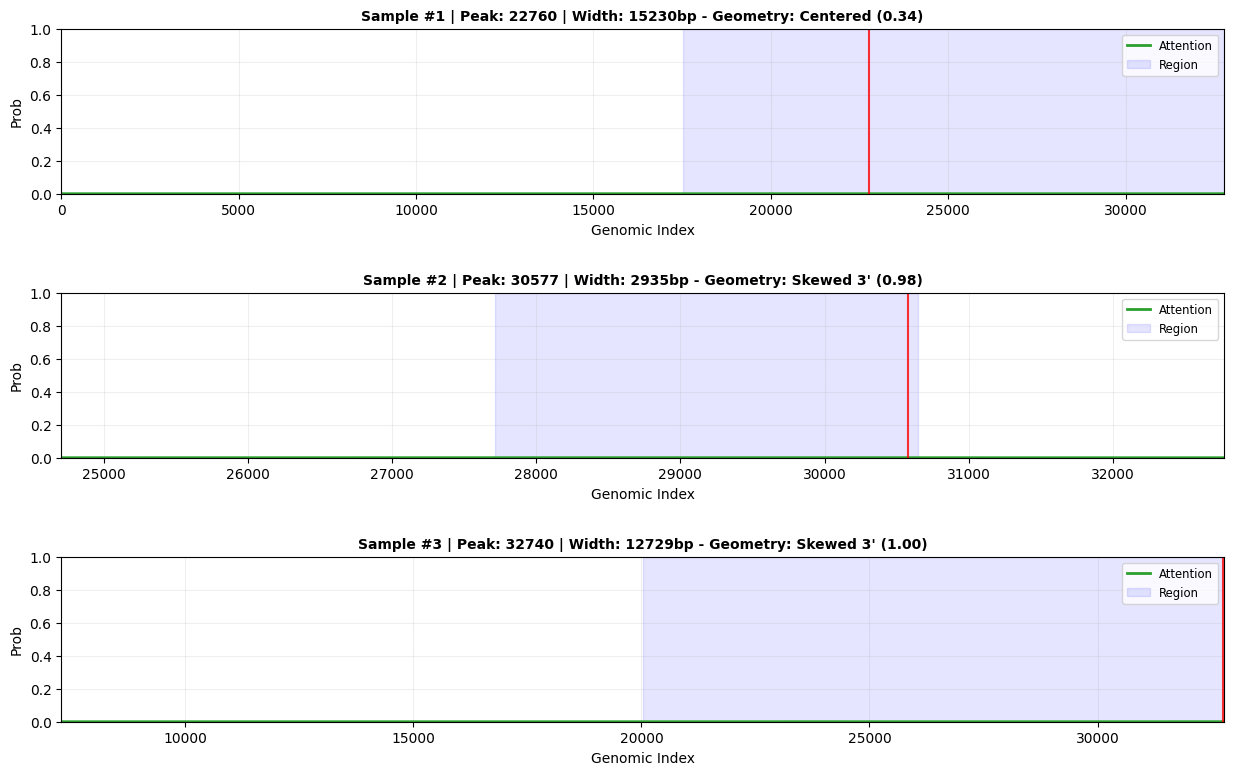
\includegraphics[width=\columnwidth]{figure4.png}}{Attention geometry}
    \begin{flushleft}
   {\textbf {Fig. 6. }\textbf{Regional Localization} The model shows diverse attention phenotypes corresponding to different breakpoint locations. (Top) A 5’-biased peak at approximate index 870 (Width: 1,808 bp). (Middle) A centered peak at approximate index 20,600 (Width: 1,855 bp). (Bottom) A 3’-biased peak at approximate index 2,000 (Width: 1,951 bp).}
    \end{flushleft}
\end{figure}
\section{Comparative Context}
\subsection{Comparison with Transformers (DNABERT \cite{dnabert}, Nucleotide Transformer \cite{nucleotide})}
Standard genomic Transformers rely on quadratic self-attention ($O(N^2)$). To mitigate computational costs, they often tokenize DNA into k-mers (e.g., 6-mers), resulting in output embeddings that represent coarse ``blocks'' rather than exact positions. While recent preliminary benchmarks suggest large foundation models can achieve high classification accuracy (e.g., for Nucleotide Transformer \cite{krupicka2025benchmarking}), they incur prohibitive latency and memory costs for long contexts. FuseLens leverages HyenaDNA's implicit long convolutions ($O(N \log N)$) to process 32\,kb windows at single-nucleotide resolution, balancing competitive accuracy with the throughput required for clinical screening.

\subsection{Comparison with CNNs (FusionAI \cite{fusionai})}
Convolutional baselines are computationally efficient ($O(N)$) but typically lack a global receptive field. Furthermore, identifying breakpoints in CNNs often requires expensive post-hoc perturbation steps (e.g., masking inputs repeatedly), where inference time scales linearly with sequence length. In contrast, FuseLens offers \textbf{intrinsic localization}: the attention weights are computed as part of the primary forward pass, yielding a breakpoint proxy at zero marginal computational cost.

\subsection{Scalability and Throughput}
While hybrid architectures like Evo (Striped Hyena) re-introduce quadratic bottlenecks via attention layers, FuseLens remains purely convolutional. Our study focuses on 32\,kb windows to capture immediate fusion boundaries, but the architecture is inherently scalable to support sequence lengths of up to 1 million base pairs, maximizing throughput for full-transcriptome analysis.

\subsection{Benchmarking Rationale}
Direct comparison with existing literature is constrain\-ed by dataset heterogeneity, preventing a strict equivalence evaluation. Baseline models are typically evaluated on limited datasets—often capping at approximately 52k samples \cite{krupicka2025benchmarking}. In contrast, we utilized the significantly larger Chimera dataset ($\sim$187k samples) to rigorously evaluate FuseLens. While this selection prioritizes granular structural validation over alignment with broader clinical benchmarks, our robust performance on this expanded scale demonstrates the model's capacity to generalize effectively across a dataset more than three times the size of standard baselines.

\section{Discussion}

\subsection{Synthetic Negatives as Constraints}
Our synthetic hard negatives serve as controlled counterfactuals designed to decouple structural grammar from gene identity. While operators like intra-gene circular permutation ($\mathcal{J}$) effectively penalize shallow edge-detection heuristics, they represent a principled training constraint rather than a comprehensive simulation of all upstream sequencing artifacts (e.g., paralog mapping ambiguity or chimeric alignments). This protocol forces the model to learn the \textit{syntax} of a fusion event rather than memorizing high-frequency chimeras.

\subsection{Localization Interpretability}
FuseLens provides an attention-derived mechanism to shortlist regions of interest at zero marginal computational cost, bridging the gap between classification speed and interpretability. By utilizing \textit{weak supervision}—deriving localization solely from binary classification labels—the model demonstrates that structural fusion features are sufficiently distinct to be spatially isolated without explicit segmentation targets. While these attention peaks are proxies, they can reduce the search space for manual validation, transforming the classifier from a black-box filter into an interpretable screening tool.

\section{Limitations and Future Directions}
\label{sec:limitations_future}

\subsection{Architectural and Input Refinements}
We identified opportunities to improve sequence boundaries and inputs. First, regarding attention dynamics, we observed an accumulation of attention peaks at the window start (see Fig. 5), acting as a probability sink. Future work will introduce an explicit "No-Op" token, preventing probability leakage. Second, the current use of random nucleotide padding—while useful for translation invariance—lacks biological context. Future work should evaluate padding with real genomic flanks to better simulate the specific noise of sequencing edges.

\subsection{Localization Precision}\label{lp-future}
The observed median resolution of 1,911 bp suggests that the model effectively captures the fusion locus, providing a strong initialization for fine-tuning. Future work will leverage the exact breakpoint coordinates inherent in the dataset to implement fully supervised segmentation heads (e.g., token-level Cross-Entropy) or semi-supervised consistency losses, directly optimizing the attention mechanism for base-pair precision.

\subsection{Clinical Integration} FuseLens can act as a post-filtering layer for upstream callers (e.g., STAR-Fusion), reducing false positive rates. It can also complement alignment-dependent long-read tools like CTAT-LR-fusion \cite{ctat_lr} by providing sequence-level robustness against mapping artifacts. Moreover, its 32\,kb window is inherently compatible with third-generation sequencing (e.g., Oxford Nanopore); future work will validate the model on uncorrected long reads, where traditional alignment faces higher error rates.

\subsection{Benchmark Alignment}
To facilitate direct comparison with emerging baselines \cite{krupicka2025benchmarking}, future work will retrain these baseline architectures on the comprehensive Chimera dataset. This expansion will quantify performance and allow FuseLens to be evaluated against the standard metrics.

\section*{Acknowledgments}
This work was supported by the Efi Arazi School of Computer Science at Reichman University. We thank the authors of HyenaDNA for providing public access to their pre-trained models.

% ================= REFERENCES =================
\begin{thebibliography}{99}

\bibitem[Ake18]{starchip}
Akers, N.K., Schadt, E.E., and Losic, B. ``STAR Chimeric Post for rapid detection of circular RNA and fusion transcripts.''
\textit{Bioinformatics}, 34(14):2364--2370, 2018. doi:10.1093/bioinformatics/bty091.

\bibitem[Dal25]{nucleotide}
Dalla-Torre, H., et al. ``The Nucleotide Transformer: Building and Evaluating Robust Foundation Models for Human Genomics.''
\textit{Nature Methods}, 2025.

\bibitem[Dru01]{imatinib}
Druker, B.J., et al. ``Efficacy and safety of a specific inhibitor of the BCR-ABL tyrosine kinase in chronic myeloid leukemia.''
\textit{New England Journal of Medicine}, 344(14):1031--1037, 2001.

\bibitem[DSo25]{chitars_db}
DSouza, D., et al. ``ChiTaRS 8.0: the comprehensive database of chimeric transcripts and RNA-seq data with applications in liquid biopsy.''
\textit{Nucleic Acids Research}, 53(D1):D1302--D1312, 2025.

\bibitem[FMe12]{chimeras_shape}
Frenkel-Morgenstern, M., et al. ``Chimeras taking shape: Potential functions of proteins encoded by chimeric RNA transcripts.''
\textit{Genome Research}, 22(7):1231--1242, 2012.

\bibitem[Gia13]{giacomini2013}
Giacomini, C.P., et al. ``Breakpoint Analysis of Transcriptional and Genomic Profiles Uncovers Novel Gene Fusions Spanning Multiple Human Cancer Types.''
\textit{PLoS Genetics}, 9(4):e1003464, 2013.

\bibitem[Haa19]{starfusion}
Haas, B.J., et al. ``STAR-Fusion: Fast and Accurate Fusion Transcript Detection from RNA-Seq.''
\textit{bioRxiv}, 2019.

\bibitem[Haa24]{ctat_lr}
Haas, B.J., et al. ``CTAT-LR-fusion: Accurate fusion transcript identification from long and short read isoform sequencing.''
\textit{bioRxiv}, 2024.

\bibitem[Jai19]{attention_not_explanation}
Jain, S. and Wallace, B.C. ``Attention is not Explanation.''
In \textit{Proceedings of NAACL-HLT 2019}, pp. 3543--3556, 2019. doi:10.18653/v1/N19-1357.

\bibitem[Ji21]{dnabert}
Ji, Y., et al. ``DNABERT: pre-trained Bidirectional Encoder Representations from Transformers model for DNA-language in genome.''
\textit{Bioinformatics}, 37(15):2112--2120, 2021.

\bibitem[Jia08]{ushuffle}
Jiang, M., Anderson, J., Gillespie, J., and Mayne, M. ``uShuffle: a useful tool for shuffling biological sequences while preserving the k-let counts.''
\textit{BMC Bioinformatics}, 9:192, 2008. doi:10.1186/1471-2105-9-192.

\bibitem[Kim21]{fusionai}
Kim, P., et al. ``FusionAI: predicting fusion breakpoint from DNA sequence with deep learning.''
\textit{iScience}, 24(12):103507, 2021.

\bibitem[Kru25]{krupicka2025benchmarking}
R.~Krupi{\v{c}}ka, M.~Kom{\'a}rkov{\'a}, B.~Dvorsk{\'y}, and O.~Klemp{\'i}{\v{r}}, ``Benchmarking genomic foundation models for gene fusion detection from DNA sequences,''
\textit{Research Square}, Dec. 2025. doi:10.21203/rs.3.rs-8360344/v1. [Preprint]

\bibitem[Kum16]{fusion_challenges}
Kumar, S., et al. ``Review of gene fusion discovery methods in cancer.''
\textit{Current Bioinformatics}, 11(4):428--438, 2016.

\bibitem[Lee23]{evoaug}
Lee, N.K., Tang, Z., Toneyan, S., and Koo, P.K. ``EvoAug: improving generalization and interpretability of genomic deep neural networks with evolution-inspired data augmentations.''
\textit{Genome Biology}, 24:105, 2023. doi:10.1186/s13059-023-02941-w.

\bibitem[Mit07]{mitelman2007impact}
Mitelman, F., Johansson, B., and Mertens, F. ``The impact of translocations and gene fusions on cancer causation.''
\textit{Nature Reviews Cancer}, 7(4):233--245, 2007.

\bibitem[Ngu23]{hyenadna}
Nguyen, E., et al. ``HyenaDNA: Long-Range Genomic Sequence Modeling at Single Nucleotide Resolution.''
\textit{Advances in Neural Information Processing Systems (NeurIPS)}, 36, 2023.

\bibitem[Pio19]{gene_length_stats}
Piovesan, A., et al. ``Gene Size Matters: An Analysis of Gene Length in the Human Genome.''
\textit{Frontiers in Genetics}, 10:1377, 2019. doi:10.3389/fgene.2019.01377.

\bibitem[Pol23]{hyena_hierarchy}
Poli, M., et al. ``Hyena Hierarchy: Towards Larger Convolutional Language Models.''
\textit{International Conference on Machine Learning (ICML)}, 2023.

\bibitem[Ren05]{bcr_abl}
Ren, R. ``Mechanisms of BCR-ABL in the pathogenesis of chronic myeloid leukemia.''
\textit{Nature Reviews Cancer}, 5(3):172--183, 2005.

\bibitem[Tom05]{tmprss2_erg}
Tomlins, S.A., et al. ``Recurrent fusion of TMPRSS2 and ETS transcription factor genes in prostate cancer.''
\textit{Science}, 310(5748):644--648, 2005.

\bibitem[Uni23]{uniprot_db}
The UniProt Consortium. ``UniProt: the universal protein knowledgebase in 2023.''
\textit{Nucleic Acids Research}, 51(D1):D523--D531, 2023.

\bibitem[Uhr21]{arriba}
Uhrig, S., et al. ``Accurate and efficient detection of gene fusions from RNA sequencing data.''
\textit{Genome Research}, 31(3):448--460, 2021.

\bibitem[Vas17]{vaswani}
Vaswani, A., et al. ``Attention is all you need.''
\textit{Advances in Neural Information Processing Systems (NeurIPS)}, 30, 2017.

\bibitem[Wie19]{attention_not_not}
Wiegreffe, S. and Pinter, Y. ``Attention is not not Explanation.''
In \textit{Proceedings of EMNLP-IJCNLP 2019}, pp. 11--20, 2019. doi:10.18653/v1/D19-1002.

\bibitem[Zen16]{zeng_dinuc}
Zeng, H., Edwards, M.D., Liu, G., and Gifford, D.K. ``Convolutional neural network architectures for predicting DNA--protein binding.''
\textit{Bioinformatics}, 32(12):i121--i127, 2016. doi:10.1093/bioinformatics/btw255.

\bibitem[Zha12]{slc45a3_elk4}
Zhang, Y., et al. ``Chimeric transcript generated by cis-splicing of adjacent genes regulates prostate cancer cell growth.''
\textit{Cancer Discovery}, 2(7):598--607, 2012.

\end{thebibliography}

\end{document}
